\chapter{TLS echoservice}

The web services of the previous chapters have one mayor drawback: the communication between the two endpoints is insecure.
For that reason the current and the next chapter will discuss how to create a secure web service.
In general, security in a network can be subdivided into the following categories:~\cite{TANNENBAUM_2001}\task{verfiy citation}
\begin{itemize}
	\item \textbf{Confidentiality} --- Protection of the data against passiv attacks (such as publicise message content)
	
	\item \textbf{Authentication} --- Verification of the Authenticity  of the communications partner.

	\item \textbf{Integrity} --- Protection against interception and manipulation,replay,insertion, etc.  of a message.

	\item \textbf{Non-repudiation} --- Preventing the sender to repudiate the message transmitted by him.

	\item \textbf{Access control} --- Restrict the access to ressources.

	\item \textbf{Availability} --- Ensure a system is always usable which is challenged by several attacks.

\end{itemize}
%1-21   Gebräuchliche Dienste
%     Identifizierung           Vermerk
%     Berechtigung              Zugriff
%     Lizenz/Zertifizierung     Gültigkeitsprüfung
%     Unterschrift              Zeitpunkt des Auftretens
%     Bezeugung                 Abstimmung
%     Übereinstimmung           Eigentum
%     Zuverlässigkeit           Registrierung
%     Quittungen                Genehmigung/Verbot
%     Bestätigung des Ursprungs Privatsphäre
%
% Nach Sicherheit in verteilten Systemen, ITM Lübeck
Ideally, all six categories should have been achieved by such an application (though the last category, availability, is difficult to realise).
In the present chapter, the security will be put into practice by extending the protocol stack with an additional security layer called TLS (Transport Layer Security).
Due to the location after the TCP and the HTTP layer, the layer is only capable to limit the access to the grid to a certain set of users.\task{What do you mean here? SM}
Nevertheless, it provides the security categories: confidentiality, authentication, integrity, non-repudiation and access control.


In the next section gives a basic understanding of the working principale of the TLS. Emphasis is put on the security concept and not on an exact description of the technical realisation in order to enable newcomers an entry to  this area.


% It is recommand to satifiy as much categories as possible. 
%authentication , confidentiality and integrity protection of TCP-based communication --- non-repudiation due to private key, access control to our service.


\section{Transport Layer Security}


The TLS is a protocol which provides a secure connection between two endpoints.
It is based directly on the TCP/IP layers and uses typically an asymmetric encryption to establish the connection (alternatively a symmetric pre-shared key may be used).
After the communication has been successfully established, both participants are switching to another encryption method which is based on a new negotiated symmetric key.
%    1. Peer negotiation for algorithm support
%    2. Key exchange and authentication
%    3. Symmetric cipher encryption and message authentication   - from wikipedia
%
%


Symmetric and asymmetric encryption are the two main classes of cryptographic algorithms.
In case of symmetric encryption, both participants are holding the same secret key to encrypt and decrypt a plain text.
The principle is to reverse the process of encryption for decrypting the text.
Symmetric encryption can be ranked as being very secure but its downside is that the key distribution is very difficult in practice.
The key has to be shared previously, ideally over a secure channel which is may either be a complete diffrent medium (i.e. a letter, speech) or a channel which has been encrypted with another secret key.
Asymmetric encryption follows a diffrent functional principle.
While the symmetric encryption utilise one shared secret, the asymmetric ecryption is based on two keys: a private key and public key.
As the names imply, the private key is kept secret and is never shared while the public key is available to everyone.
Messages encrypted with the public key can only be decrypted with the private key and conversely, messages encrypted with the private key can only be decrypted with the public key. 
The Figure~\ref{fig:asymmetric_encryption} illustrates the circumstances of the case.
\begin{figure}[htb]
	\centering%epstopdf async.eps
	\subfloat[Texttext\label{fig:cgd}]
		{\includegraphics[width=12cm]{tex_tls_echoservice/async.pdf}}\\
	\subfloat[Texttext\label{fig:cgd}]
		{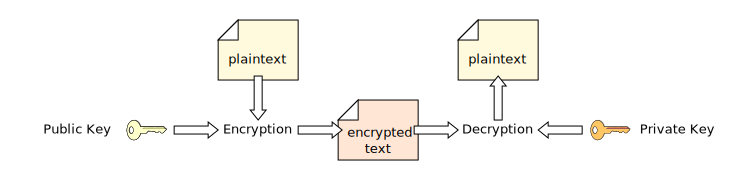
\includegraphics[width=12cm]{tex_tls_echoservice/async2.pdf}}
	\label{fig:asymmetric_encryption}
	\mycaption{specific}{general}
\end{figure}
\task{Maybe the term service has to be replaced by server}

At startup of the communication process, A (Alice) who desires a secure connection transmits her public key to B (Bob).
Bob is now able to encrypt his messages such that only Alice is able to decrypt them.
As one can see, this first approach already provides confidentiality and integrity of messages.

Neither Non-repudiation, authentication and consequently nor access control are established because the identity of Alice is not proven.
In order to be able to check identities, so called certificates have been introduced.
Certificates render the possibility to validate the identity of its owner.
They are signed by a certificate authority (CA), the identity of which can be verified by another CA or that is pre-configured to be trusted.

A certificate is composed of the identity of the owner, his public key, the name of the CA who signed the certificate and the signature of the CA which is a hash-value of the certificate encrypted with the private key of the CA. 
Furthermore, the algorithms used to create the certificate are added.
If a certificate can be resolved to a trusted CA, the identity of the certificate owner is considered to be proven. 
In general, a set of trusted CAs is already defined in the operation system.
To obtain a certificate, a certificate request has to be submitted to a CA.
The CA verifies the identity of the requesting person and the requested certificate will be signed.
Figure~\ref{fig:certificate_request} shows the procedure of gaining a certificate.
For instructions on the actual commands on the UNIX shell, you may follow instructions on \url{http://ca.nordugrid.org}.
\begin{figure}[htb]
	\centering%epstopdf certificates.eps
 	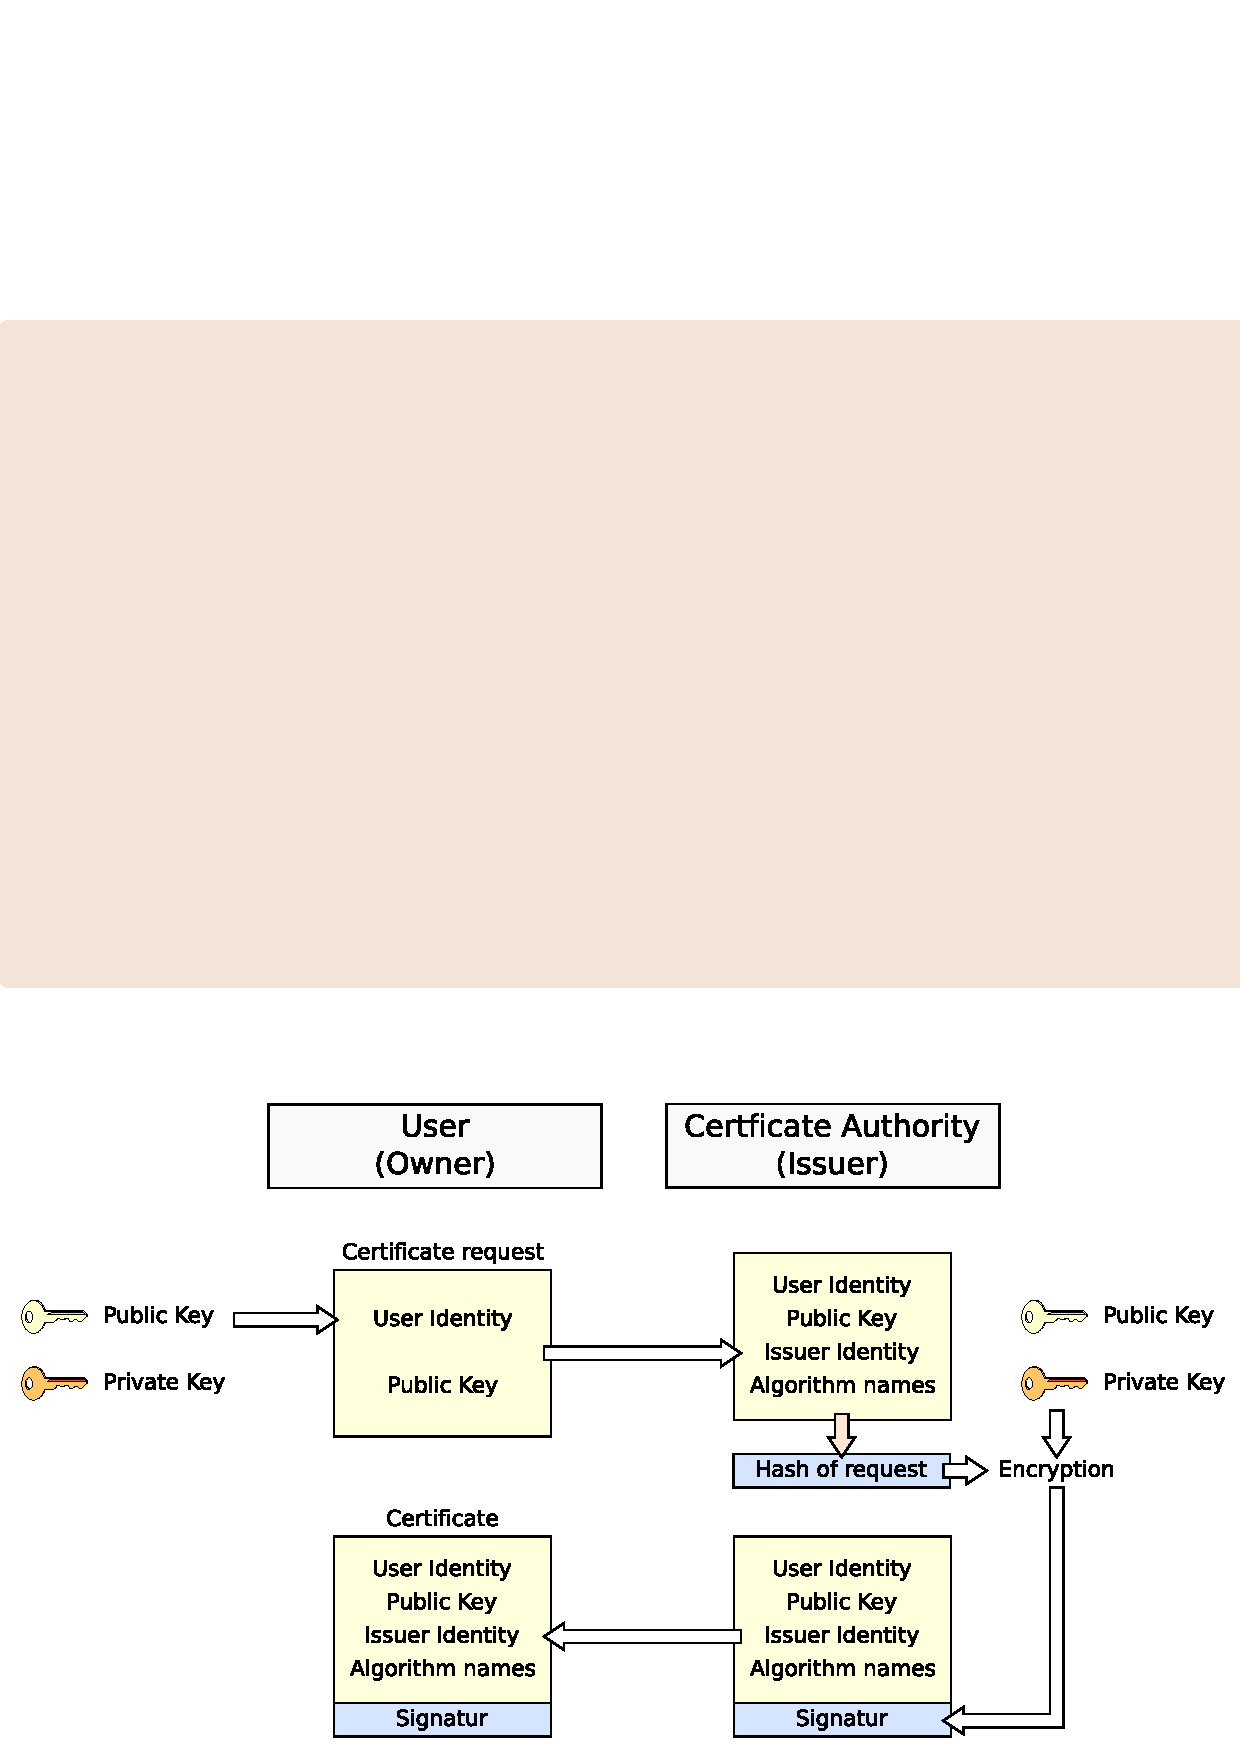
\includegraphics[width=13cm]{tex_tls_echoservice/certificates.pdf}
	\mycaption{specific}{general}
	\label{fig:certificate_request}
\end{figure}
In the first step, a private and a public key will be generated by the requester.
The public key together with a textual description of the identity depict the request which will be transmitted to a CA.
After the CA successfully verified the validity of the request, the identity of the CA and the name of the used encryption algorithms are added.
The collected data will represent the plain text of the certificate.
In order to ensure the integrity of the text, a hash value will be created.
This is a fixed-sized short string which is generated by an algorithm based on an arbitrary long given text.
The algorithm is designed such that a small change in the text will cause the hash value to change almost like a random function.
Thus, the hash value can be used a fingerprint of the text.
The CA signs the plain certificate by encrypting its hash value with its private key.
Finally the signed certifcate will be returned to the requester.
If an outside person wants to verify the certificate owner, the encrypted hash value has to be decrypted by the public key of the CA and a hash value has to be created with the same algorithm in order to compare them.


Figure~\ref{fig:verification_of_certificates} shows a usecase in which Alice wants to resolve the identity of Bob.
Alice submits her request to Bob along with a challange consisting of a random number $n$. 
The random number ensures that it is not possible to repeat a message (integrity).
Bob encrypts the number with his private key and returns it together with his certificate.
Alice uses the public key of Bob to decrypt the challenge. 
If the decrypted number is equal to the transmitted number, Alice can reason that the identity of Bob is to be trusted in case she is trusting the CA which has signed Bobs certificate. 

In the given example, Alice only trusts the CA 2 but not CA 1.
To resolve the identity of CA 1, Alice establishes a connection to CA 1 and submits another random number $n$ as a challenge.
The CA 1 encrypts the challenge with its private key and sends the result along with its certificate back to Alice.
Alice successfully validates the certificate of CA 1.
Since the certificate was signed by CA 2 which is pre-configured to be trusted, she als trusts CA 1 and in conclusion the identity of B.
In summary, Alice knows she is talking to Bob.
If Bob also wants to be sure who he's talking to, then the same procedure has to be done to confirm the identity of Alice.
The TLS mode in which both endpoints are ensuring themselves to whom they are talking to is called \textit{bilateral connection mode}.


When the client is aware of the service authentity, the confidential treatment of his data is given such that one can be sure the data won't be revealed to a third party (service-sided confidentiality). 
On the other side, if the service is aware of the client authentity, the access to the service can be controlled (access control) and the service can verify that the results will only be passed back to the right person (client-sided confidentiality). 
As one can see confidentiality, authentication, integrity and non-repudiation are now given.

\begin{figure}[htb]
	\centering%epstopdf verification.eps 
	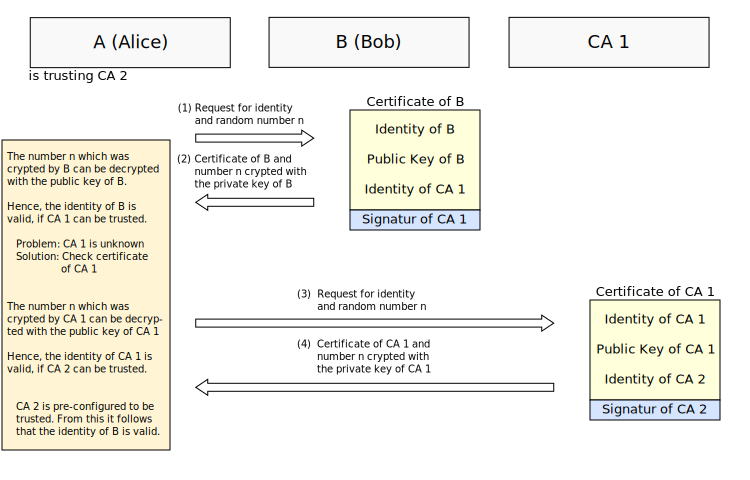
\includegraphics[width=13cm]{tex_tls_echoservice/verification.pdf}
	\mycaption{specific}{general}
	\label{fig:verification_of_certificates}
\end{figure}

Certificates have several advantages.
They are scaling very good with the amount of users because CAs can create new sub-CAs such that the load is balanced (certificates of a CA may be cached).
Furthermore no critical information is exchanged during the establishment of a connection (in particular no secret key is shared which may get intercepted).
Instead, a set of pre-configured CAs which will be in general provided by the operation system is needed.
In respect of ARC it is obvious that the access to the grid shall be under control of its administrator.
To do so, the administrators have to establish their own CA such which is in charge of creating certificates for a set of users.
Many universities have prepared local certificate authorities.
And every user can establish his own. 

The identity of the created CA have to be added to the directory of pre-configured CAs.
The ARC source code comes with two shell scripts to create a CA and related certificates.
Several publicly availble tools for certificate handling haven been prepared, e.g. (like \textit{openssl}),
which allow the certificate handling also for the advanced UNIX users.
Certificates in general, however, have found entry to regular computer users, for instance with the FernUniversity Hagen (https://ca.fernuni-hagen.de/) who use that technology for their remote students to hand in exercises.

A CA which controls the access to a grid can be considered as a virtual organsiation (VO).
It may involve organisations close to the leading organisation as well as structure which are not formally associated with it.
In most cases the basic idea is to share ressources. \task{this para will need some overhaul - SM}

\clearpage
\section{Service}
\task{RENAMING HED configuration file into~ARC service configuration file - proposed by Marek}
\task{(echo service) client configuration file - proposed by Marek}

In order to create a secure bilateral connection we hence need two certificates: a client certificate and a service certificate.
The CA for the certificate has to be pre-configured on the counterpart and furthermore, the owner of the certificate has to hold the fitting private key.
For the given example X.509-certificates will be used which are standardised by the ITU-T.
Altogether six files are needed:
\begin{tabular}{l@{~---~}p{13cm}}
\textbf{clientCA}   & The CA which guarantees for the identity of the client \\
\textbf{clientCERT} & The certificate of the client. \\
\textbf{clientKEY}  & The private key of the client (should be kept in safe custody).\\
\\
\textbf{serverCA}   & The CA which guarantees for the identity of the server \\
\textbf{serverCERT} & The certificate of the server. \\
\textbf{serverKEY}  & The private key of the server (should be kept in safe custody).\\
\end{tabular}
\forcelinebreak
As one can see, PEM has been choosen for the file format.\\

To get this service running, the six files have to be distributed. The server should hold the files: serverCERT.pem, serverKEY.pem and clientCA.pem. The client on the other side should own the files: clientCERT.pem, clientKEY.pem and serverCA.pem.
Within the source code directory certificates with corresponding names are prepared. Due to certificates have a limited period of validity, these certificates may no longer be accepted by the communication parter. In order to create a first basic set of certificates signed by a self created CA, the shell scripts \textit{createMasterCA.sh} and \textit{createSlaveCert.sh} to be found in the directory \textit{src/services/tlsechoservice/certFactory} may be used. The script \textit{createMasterCA.sh} will create a new CA and overwrite the old on which was stored in the directory. The script \textit{createSlaveCert.sh} create an arbitary amount of certificates signed by the CA which has been create by the other script.\\
%WARNING: If the programm fails, check if one of your certifacte is expired. If so, create new one using the script files in the directory 'certFactory'


The TLS echo service implementation is almost the same as the one presented in the chapter before. Merely the Class name and the namespace of the service has changed. The only modification has to be done within the ARC service configuration file which is displayed in Listing~\ref{lst:tls_echo_arched_xml}.

\lstsetARCHEDXML
\lstinputlisting
	[
	label=lst:tls_echo_arched_xml,float=htb,
	caption={[HED configuration file for the Arc intern echo service. Filename: arcecho\_no\_ssl.xml]
	\textbf{HED configuration file for the Arc intern echo service. Filename: arcecho\_no\_ssl.xml\textcolor{white}{hmf}}}
	]
{../src/services/tlsechoservice/arched_tls_echoservice.xml}
The first change is to be found in lin~\ref{lst_code:tls_echo_arched_xml_plugin}. As to be seen, another plugin called \textit{mcctls} will be loaded by the \textit{ModuleManager}. The second change is the new element which has been placed between the TCP and the HTTP component, see line~\ref{lst_code:tls_echo_arched_xml_component}. Within the element the files are declared using the elements
\begin{verbatim}
<KeyPath>./clientKey.pem</KeyPath>
<CertificatePath>./clientCert.pem</CertificatePath>
<CACertificatePath>./serviceCA.pem</CACertificatePath>
<CACertificatesDir>/etc/grid-security/certificates</CACertificatesDir>
\end{verbatim}
or
\begin{verbatim}
<ClientSSLConfig FromFile='filename'/>
\end{verbatim}
\task{You can put the ClientSSLConfig into a separate file, then use <ClientSSLConfig FromFile='filename'/> in each service, and then you don't need to change everywhere - proposed by Zsombor}


%\lstsetCPP
%\lstinputlisting
%	[
%	label=lst:tls_echo_service_cpp,
%	caption={[HED configuration file for the Arc intern echo service. Filename: arcecho\_no\_ssl.xml]
%	\textbf{HED configuration file for the Arc intern echo service. Filename: arcecho\_no\_ssl.xml\textcolor{white}{hmf}}}
%	]
%{../src/services/tlsechoservice/tlsechoservice.cpp}
%
% Lassen wir mal weg....
%
%
% \lstsetKSH
% \begin{lstlisting}[
% label=lst:tls_echo_arched_invoke,float=htb,
% caption={[Transformation in eine uniforme konzentrische Verteilung.]
%          \textbf{Transformation in eine uniforme konzentrische Verteilung.\textcolor{white}{hmf}}}]
% $ rm -f /var/log/arched.log
% $ arched -c arched_echoservice.xml  && echo jo ||echo n
% $ tail -n100 -f /var/log/arched.log
% $ killall arched
% \end{lstlisting}
% 
%        ...das auch.....


\clearpage
\section{Client}

In this section a new way to implement the client will be introduced. As already mentioned in section~\ref{sec:timeservice_client}, the protocol stack of the client is build up in almost the same way like the service. Indeed, the class~\textit{ClientSOAP} composes the stack with the same MCC used for the service. Once this is known, its self-evident to create the client in a simlar manner like the service with an own configuration file.
Listing~\ref{lst:tls_echo_client_cpp} shows the C++ source code of the client implementation. The main difference between the simple echo client presented in the chapter before is that now the information about the client protocal stack is encapsulated within a configuration file.
\lstsetCPP
\lstinputlisting
	[
	label=lst:tls_echo_client_cpp,
	caption={[HEC configuration file]
	\textbf{HEC configuration file\textcolor{white}{hmf}}}
	]
{../src/clients/tlsechoclient/tlsechoclient.cpp}
The file containing the client configuration is specified within the command line. 
Its content will be loaded in the code fragment starting in line~\ref{lst_code:tls_echo_client_cpp_getfilecontent}. 
Later, in line~\ref{lst_code:tls_echo_client_cpp_loadconfiguration}, the configuration will be parsed into XML and than transfered into a chain of component which is wrapped by the object \textit{loader}. In order to process a message, an entry point within the chain has to be disclosed. For we are implementing a SOAP client, we are looking for the SOAP component. 
To get the proper component an operator of MCCLoader is used in line~\ref{lst_code:tls_echo_client_cpp_cliententry}.
The previously used class \textit{ClientSOAP} has eased some workload which now has to be done within the method.
The payload now have to be wrapped by the message class which have to be initialised with an \textit{MessageAttribute} object and a \textit{MessageContext} object. After the payload has been wrapped within the message it gets transmitted in almost the same way like before, see lines followed by line~\ref{lst_code:tls_echo_client_cpp_createandprocess}. The rest of the source code is identical to the echo client.\\





% Folgender XML Aufruf und Antwort soll \textit{automatisch} generiert werden:






% 
% \lstsetJUSTXML
% \begin{lstlisting}[
% label=lst:tls_echo_request_XML,float=htb,
% caption={[Transformation in eine uniforme konzentrische Verteilung.]
%          \textbf{Transformation in eine uniforme konzentrische Verteilung.\textcolor{white}{hmf}}}]
% <soap-env:Envelope xmlns:tlsecho="urn:tlsecho" xmlns:soap-enc="http://schemas.xmlsoap.org/soap/encoding/" xmlns:soap-env="http://schemas.xmlsoap.org/soap/envelope/" xmlns:xsd="http://www.w3.org/2001/XMLSchema" xmlns:xsi="http://www.w3.org/2001/XMLSchema-instance">
%   <soap-env:Body>
%     <tlsecho:tlsechoRequest>
%       <tlsecho:say operation="ordinary">text_to_be_transmitted</tlsecho:say>
%     </tlsecho:tlsechoRequest>
%   </soap-env:Body>
% </soap-env:Envelope>
% \end{lstlisting}
% 
% 
% 
% 
% 
% 
% \lstsetJUSTXML
% \begin{lstlisting}[
% label=lst:tls_echo_response_XML,float=htb,
% caption={[Transformation in eine uniforme konzentrische Verteilung.]
%          \textbf{Transformation in eine uniforme konzentrische Verteilung.\textcolor{white}{hmf}}}]
% <soap-env:Envelope xmlns:tlsecho="urn:tlsecho" xmlns:soap-enc="http://schemas.xmlsoap.org/soap/encoding/" xmlns:soap-env="http://schemas.xmlsoap.org/soap/envelope/" xmlns:xsd="http://www.w3.org/2001/XMLSchema" xmlns:xsi="http://www.w3.org/2001/XMLSchema-instance">
%   <soap-env:Body>
%     <tlsecho:tlsechoResponse>
%       <tlsecho:hear>[ text_to_be_transmitted ]</tlsecho:hear>
%     </tlsecho:tlsechoResponse>
%   </soap-env:Body>
% </soap-env:Envelope>
% \end{lstlisting}
% 
